\tightsection{Quality Improvement via Prediction}
\label{improvement}
Now we can fill in the details of section 3 a bit more.  Figure~\ref{fig:go-overview} shows how prediction and decision-making work in GO.
\fillme


\begin{figure}[h!]
\centering
 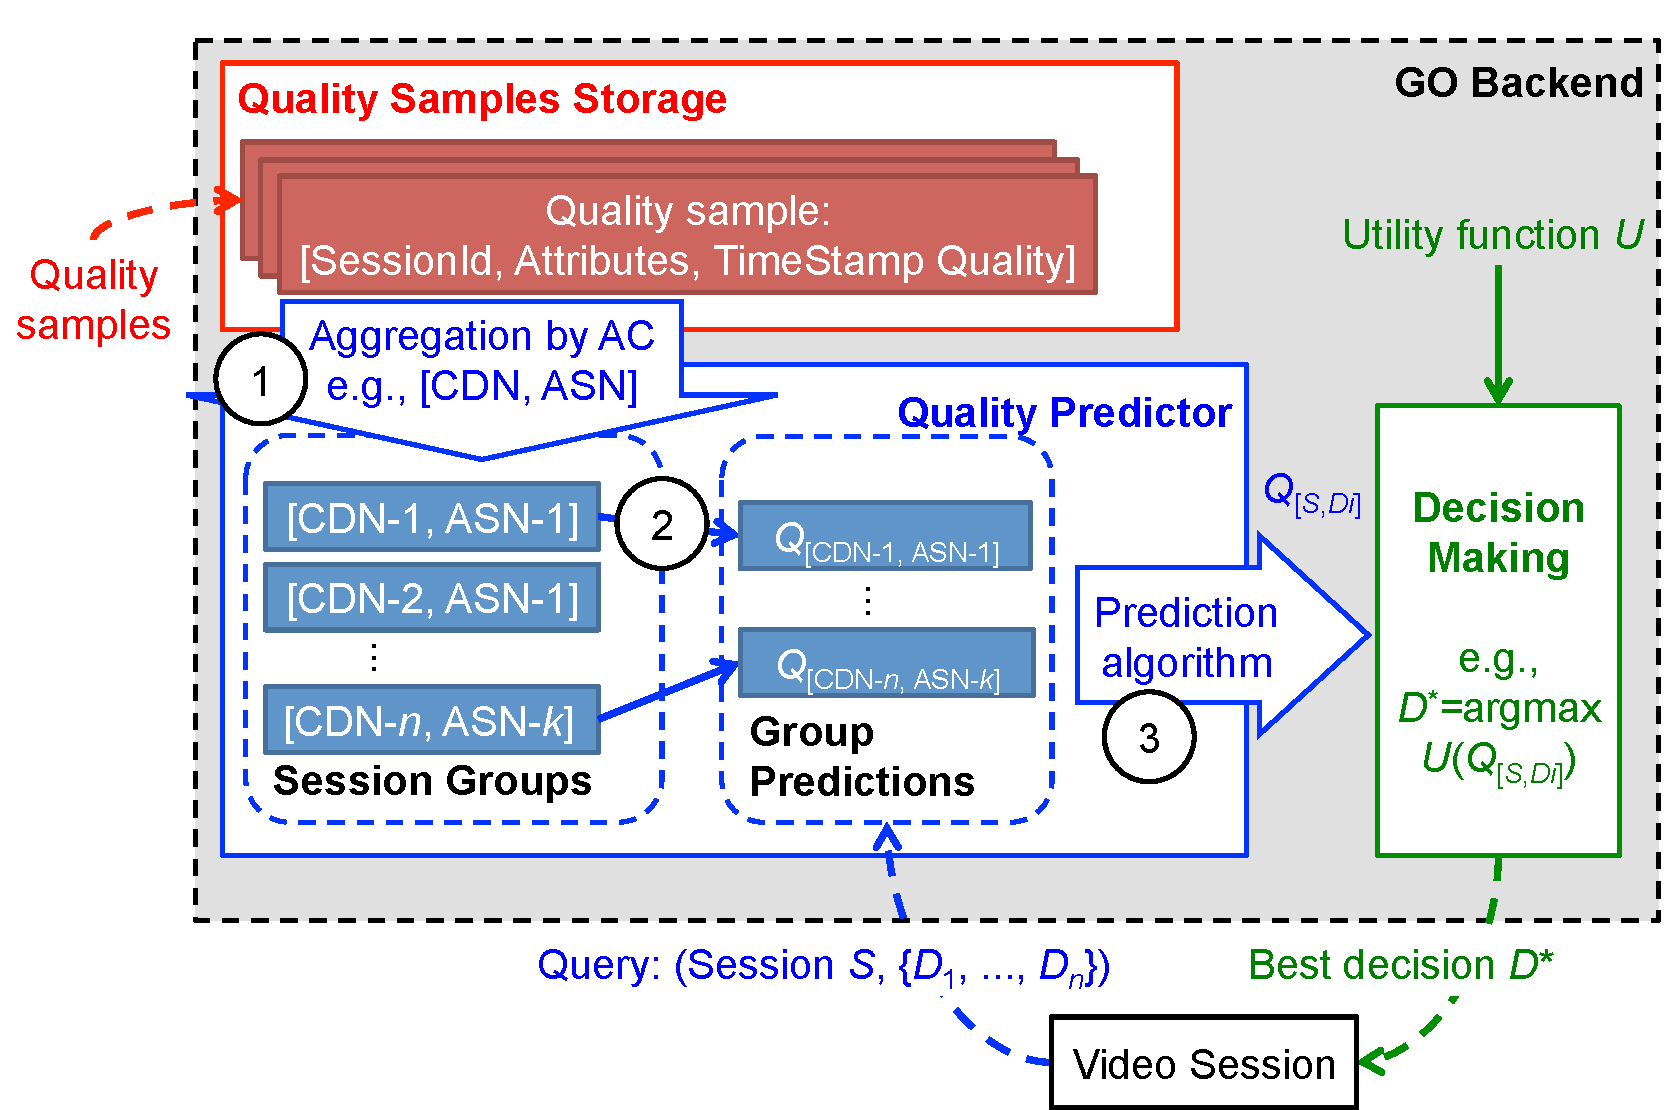
\includegraphics[width=0.5\textwidth] {figures/backend.pdf}
\tightcaption{Schematic overview of GO backend.}
\label{fig:backend}
\end{figure}

\tightsubsection{Improving quality with GO}

\tightsubsubsection{Behavioral study}
To build confidence in this algorithm, we show how decision-making based on prediction behaves in some simple synthetic scenarios where the optimal decisions are clear:
\begin{packedenumerate}
  \item A sudden change in CDN performance causes relative performance to change.
  \item One CDN performs better for one group (under an observed attribute) and worse for another group.
  \item As above, CDN performance is heterogeneous across groups, and the number of groups and sparsity of quality samples within each group is varied.
\end{packedenumerate}
\fillme

\tightsubsubsection{Evaluation against a baseline using real data}
We show how GO works in practice in a real trace, in comparison to a naive baseline algorithm that makes random decisions.  Here we use a methodology similar to A/B testing, which we call {\it counterfactual testing}; the methodology is described in detail in section \ref{sec:counterfactualtesting}.  The dataset is described in section \ref{subsec:dataset}.  Results are displayed in figure \fillme; we can see that \fillme.

\tightsubsubsection{Synthetic dataset methodology}
Randomized experimentation in real traces is the most important way to evaluate a decision-making algorithm.  However, real traces have a few limitations.  In real traces, it is impractical to identify an optimal alternative against which to compare GO, so that we can understand how close it is to the best algorithm.  In addition, real traces do not admit simple analysis of the sensitivity of a decision-making algorithm to the rapidity of changes or the degree of heterogeneity.  To remedy these limitations, we generate a synthetic dataset from our real data.  We do this using a simplifying assumption: We fix a set of attributes $g$, and assume that conditional on a session belonging to a group under this AC, its quality outcomes given each decision are statistically independent.  Essentially this amounts to an assumption that we observe all interesting attributes.  \fillme.

Under this assumption, we can generate a new session from the same distribution that generated a real dataset as follows: Sample uniformly at random from the sessions we observed.  The synthetic session has the same attributes, denoted $a_i$, as the sampled session.  We assign quality outcomes to each possible decision by sampling uniformly at random from the quality outcomes observed for sessions with attributes exactly matching $a_i$.  Crucially, this ensures that quality outcomes in the synthetic scenario are known for any decision, not just the decision that was actually taken for a session.  In particular, it is possible to identify an {\it oracle} for this scenario that makes perfect predictions of quality outcomes for any decision.

% [The following is an unfinished writeup for old synthetic scenario scheme:]
%The scenario is generated as follows: The scenario lasts for $T$ minutes.  Each session is assigned values on four different attributes, $A_0, A_1, B_0,$ and $B_1$, and lasts for $1$ minute.  Each unique attribute combination (i.e. each group) $a$ is associated with some static parameters and some parameters that change over time, which inform the generation of sessions in that group:
%\begin{packedenumerate}
%  \item $n_{a}$: The number of sessions in this group.
%  \item $\mu_{atj}$: The average quality outcome for sessions in this group, when decision $j$ is taken.
%  \item $\sigma_{atj}$: The standard deviation of quality outcomes for sessions in this group, when decision $j$ is taken.
%\end{packedenumerate}
%
%For each minute $t$, sessions are generated as follows: Group $a$ has $n_{a}$ sessions.  The $i$th session in group $a$ has attribute values $a$.  There are $J$ possible decisions; each session has quality outcome $q_{itaj}$ drawn from the distribution $\operatorname{Normal}(\mu_{atj}, \sigma_{atj}^2)$, for each decision $j$.  The actual decision $d_{ita}$ for the session, which is used to populate the quality sample used in GO, is chosen uniformly at random from among the $J$ possible decisions.

\tightsubsubsection{Evaluation against an oracle using synthetic data}
Here we compare GO against the oracle (and against a random decision-maker) in our synthetic scenario. \fillme

\tightsubsection{Understanding the impact of prediction accuracy on quality improvement}

Separately from the GO algorithm, it is also interesting to see how prediction error generically impacts quality outcomes.  Here it is important to identify an oracle predictor as a baseline, so we use the same synthetic scenario as above.  We add random independent Gaussian noise to the oracle's predictions (an admittedly crude model of prediction error) and show how larger amounts of noise impact quality outcomes.  Figure \fillme displays this.  We can see that quality improvement is unaffected by small amounts of prediction inaccuracy but drops off quickly at a (scenario-dependent) threshold \fillme.

We cannot subtract noise from GO's predictions in a real scenario, since we do not know the true outcome of decisions we did not take.  However, we can {\it add} noise to GO's predictions and observe the impact of {\it worse} prediction on quality outcomes.  As above, we use independent random Gaussian noise of varying magnitude.  Figure \fillme displays this for our synthetic scenario, and figure \fillme displays it for a real trace.  In the synthetic scenario, GO's performance in quality improvement is equivalent to that of an oracle with \fillme random noise.  \henry{We hope to see that decreasing prediction accuracy eventually leads to highly degraded performance.}